\section{Оборудование и инструментальные погрешности}

\begin{figure}[h!]
    \center{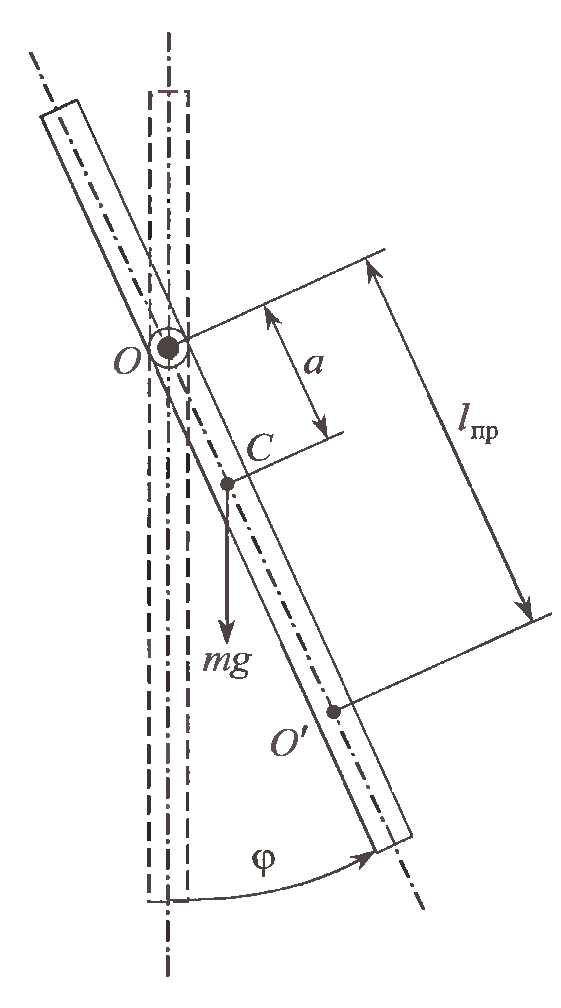
\includegraphics[width=0.8\linewidth]{img/equipment.png}}
\end{figure}

Схема установки приведена на рисунке. На стержне закрепляется опорная призма,
острое ребро которой является осью качания маятника. Призму можно перемещать
вдоль стержня., меняя расстояние $OC$ от центра масс до точки опоры, $\left|OC\right|=a$.

Момент инерции маятника
\[I=\frac{ml^2}{12}+ma^2,\]
$m$~--- масса маятника, $l$~--- длина стержня.

Момент силы тяжести
\[M=-mga\sin\varphi\approx -mga\varphi\]

Затухание маятника слабо, поэтому моментом сил трения можно пренебречь.

Уравнение колебаниий
\[\ddot{\varphi}+\omega^2\varphi=0\]

Частота колебаний
\[\omega^2=\frac{ga}{a^2+l^2/12}\]

Период 
\[T=\frac{2\pi}{\omega}=2\pi\sqrt{\frac{a^2+l^2/12}{ga}}\]

$l_\text{пр}=a+\frac{l^2}{12a}$~--- приведённая длина физического маятника.
Точка $O'$ на расстоянии $l_\text{пр}$ от $O$ называется центром качания.
Периоды колебаний при опорах в точках $O$ и $O'$ совпадают.

\begin{table}[]
    \caption{Погрешности оборудования}
    \begin{tabular}{|l|l|l|}
    \hline
    Оборудование   & $\sigma$            & $\varepsilon$       \\ \hline
    Штангенциркуль & $0{,}05\,\text{мм}$ & $5\cdot10^{-5}$     \\ \hline
    Линейка        & $0{,}5\,\text{мм}$  & $2{,}5\cdot10^{-3}$ \\ \hline
    Секундомер     & $0{,}005\,\text{с}$ & $1{,}7\cdot10^{-4}\,\text{(за 20 колебаний)}$ \\ \hline
    Весы           & $0{,}05\,\text{г}$  & $6{,}6\cdot10^{-4}$ \\ \hline
    \end{tabular}
\end{table}

Определим вклад инструментальных погрешностей в ответ.
\[g=4\pi\frac{a^2+l^2/12}{t^2a}\]
\[\varepsilon_g=\sqrt{\left(2\varepsilon_a\right)^2+\left(2\varepsilon_l\right)^2+\left(\varepsilon_a\right)^2\left(2\varepsilon_t\right)^2}=
\sqrt{\left(\sqrt{5}\varepsilon_a\right)^2+\left(2\varepsilon_l\right)^2+\left(2\varepsilon_t\right)^2}\]

\begin{gather*}
    \sqrt{5}\varepsilon_a\approx 5\cdot10^{-3} \\
    2\varepsilon_l\approx 10^{-4}
\end{gather*}
тогда
\[2\varepsilon_t\approx 5\cdot10^{-3}/2\]
\[\varepsilon_t\approx 10^{-3}\]

